\chapter{Results}

\section{Introduction}

This chapter presents the results of the experiments conducted in the previous chapter. 
The results are presented in the form of figures, tables, and descriptions.

\section{Hit Ratio Per Cache Size Experiment}

This section presents the results of the hit ratio per cache size experiment for each dataset.

\subsection{BrightKite Dataset}

The hit ratio per cache size per tenant for the BrightKite dataset is shown in Figure 
\ref{fig:hit_ratio_per_cache_size_exp_brightkite}.

The penalty function score (fault score) per cache size for the BrightKite dataset 
is shown in Table \ref{tab:fault-score-per-buffer-size-brightkite}.

By comparing LRU with Fault Ratio with Cache Used Policy (LRU in Figure and Table) with LRU 
using Naive Policy (NaiveLRU in Figure and Table), we observe that the Fault Ratio with Cache 
Used Policy improves with a higher cache size, performing similarly or worse with smaller cache 
sizes, but better with larger cache sizes, outperforming the NaiveLRU policy for all tenants 
after a cache size of 125.

We observe that most of the cache eviction policies perform well with the Fault Ratio with 
Cache Used Policy, many of them outperforming separate or naive LRU policies with a 20\% 
higher cache size (since they show a 0 penalty score) for different cache sizes.

LRU-2, LIRS, and MQ perform particularly well, showing a 0 penalty score for all cache sizes of 
125 or higher and high hit ratios for all tenants. LIRS results are particularly interesting 
since it is a low-overhead policy, and LRU-2 is performing very well.

\newpage

\begin{figure}
    \centering
    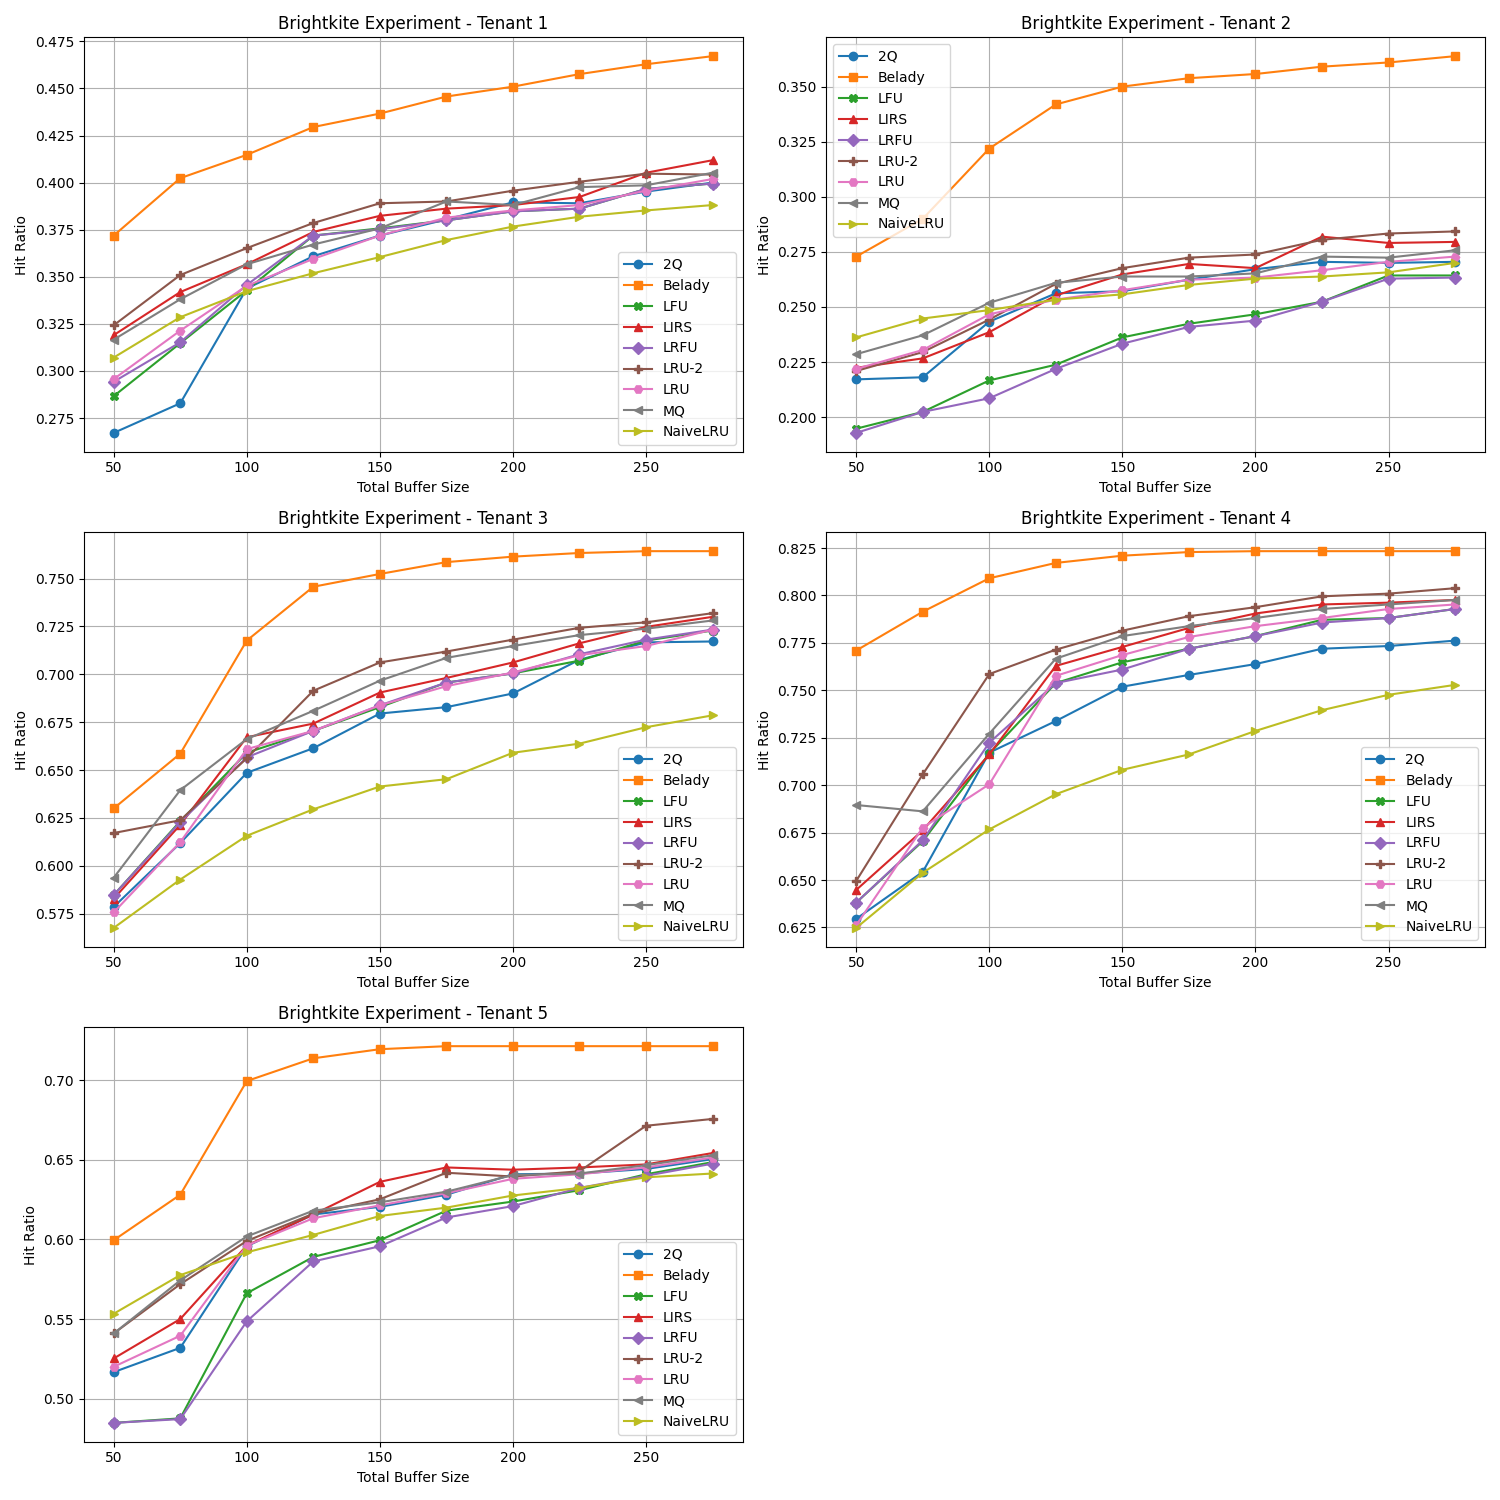
\includegraphics[width=0.75\textwidth]{hit_ratio_per_cache_size_exp_brightkite.png}
    \caption{Hit ratio per cache size per tenant for the BrightKite dataset}
    \label{fig:hit_ratio_per_cache_size_exp_brightkite}
\end{figure}

\begin{table}[ht]
    \centering
    \small
    \caption{Penalty function score (fault score) per cache size for the BrightKite dataset}
    \csvautotabular{data/fault_score_per_buffer_size_brightkite.csv}
    \label{tab:fault-score-per-buffer-size-brightkite}
\end{table}

\newpage

\subsection{CitiBike Dataset}

The hit ratio per cache size per tenant for the first experiment with the CitiBike dataset is
shown in Figure \ref{fig:hit_ratio_per_cache_size_exp_citibike}.

The penalty function score (fault score) per cache size for the first, second and third 
experiments with the CitiBike dataset are shown in Tables 
\ref{tab:fault-score-per-buffer-size-citibike}, \ref{tab:fault-score-per-buffer-size-citibike-2}
and \ref{tab:fault-score-per-buffer-size-citibike-3} respectively.

In the first experiment, we observe that most of the cache eviction policies perform very 
well with the Fault Ratio with Cache Used Policy, many of them outperforming separate or 
naive LRU  policies with a 20\% higher cache size (since they show a 0 penalty score) for 
different cache sizes.

In other experiments, results are not as good as in the first experiment, still showing
good results and low penalty scores with several cache eviction policies.

LFU, LRU-2, LIRS, and MQ perform particularly well, showing a 0 penalty score for most cache 
sizes. LIRS results are particularly interesting since it is a low-overhead policy, 
and LFU is performing very well. 

Note that even though LFU is performing very well in this dataset, it is not practical in some 
real-world scenarios since it suffers greatly from access pattern changes.

\newpage

\begin{figure}
    \centering
    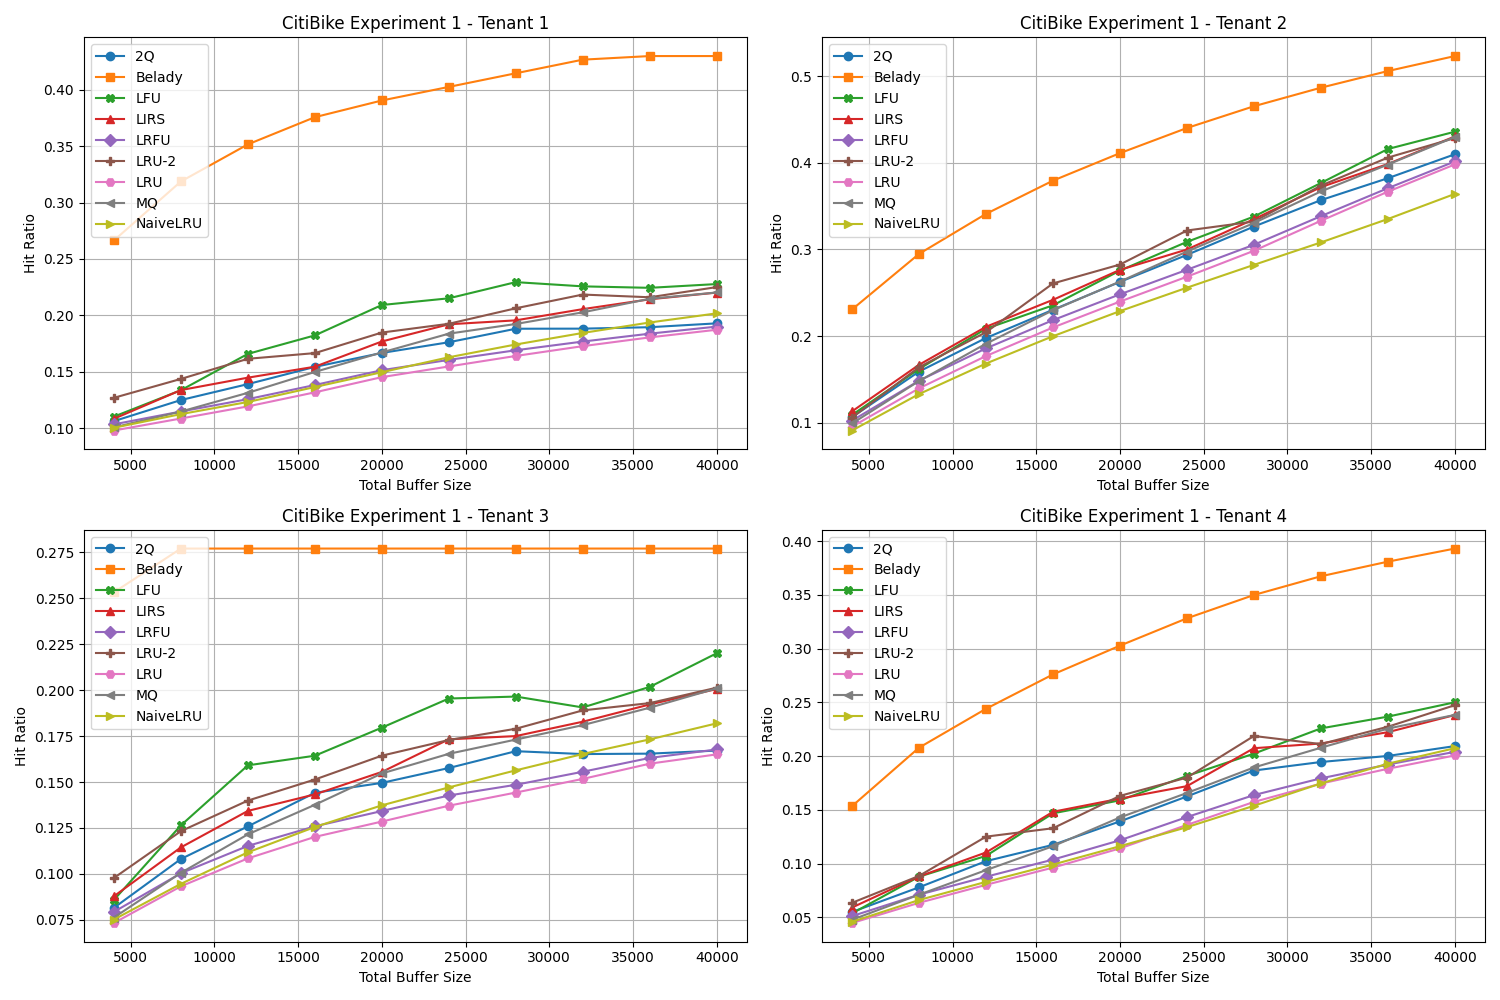
\includegraphics[width=0.75\textwidth]{hit_ratio_per_cache_size_exp_citibike.png}
    \caption{Hit ratio per cache size per tenant for the CitiBike dataset (first experiment)}
    \label{fig:hit_ratio_per_cache_size_exp_citibike}
\end{figure}

\begin{table}[ht]
    \centering
    \small
    \caption{Penalty function score (fault score) per cache size for the CitiBike dataset (first experiment)}
    \csvautotabular{data/fault_score_per_buffer_size_citibike_1.csv}
    \label{tab:fault-score-per-buffer-size-citibike}
\end{table}

\begin{table}[ht]
    \centering
    \small
    \caption{Penalty function score (fault score) per cache size for the CitiBike dataset (second experiment)}
    \csvautotabular{data/fault_score_per_buffer_size_citibike_2.csv}
    \label{tab:fault-score-per-buffer-size-citibike-2}
\end{table}

\begin{table}[ht]
    \centering
    \small
    \caption{Penalty function score (fault score) per cache size for the CitiBike dataset (third experiment)}
    \csvautotabular{data/fault_score_per_buffer_size_citibike_3.csv}
    \label{tab:fault-score-per-buffer-size-citibike-3}
\end{table}

\newpage

\section{Fault Score Experiment}
